\chapter{State of the art modelling of comfort}
\label{cha:Literature_study}

As discussed in the introduction the goal of the thesis is to learn and implement a method to capture personal experience of comfort in autonomous driving. This will be done by using an inverse optimal control approach where the weights are learned from demonstration. To be able to do this it is necessary that a literature study is done about how to define comfort in a vehicle and to gain information about inverse optimal control.\\
This chapter will give an overview of the literature that is available and will show how the thesis fits in earlier conducted research.

\section{What are the parameters that define comfort during driving?}\label{s:comfort_parameters}
In the following US patent \cite{Daniel2018} the idea is to assess the amount of comfort by calculating a value for carsickness. This value is calculated by a weighted sum of the sway motion, surge motion and heave motion of the vehicle. These motions are being directly calculated from the lateral acceleration, fore-aft acceleration and the vertical acceleration of the vehicle. \\

\begin{figure}[h!]
	\centering
	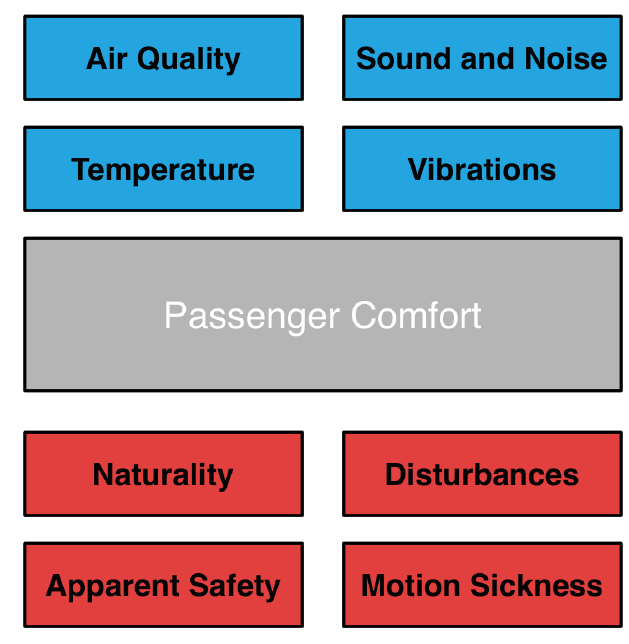
\includegraphics[width=0.48\textwidth]{comfort.PNG}
	\caption{Overview of comfort parameters in autonomous vehicle with old parameters (blue) and new ones (red).(Source: \cite{Elbanhawi2015})}
	\label{fig:Comfort}
\end{figure} 

%\begin{wrapfigure}[22]{L}{0.5\textwidth}
%	\begin{center}
%		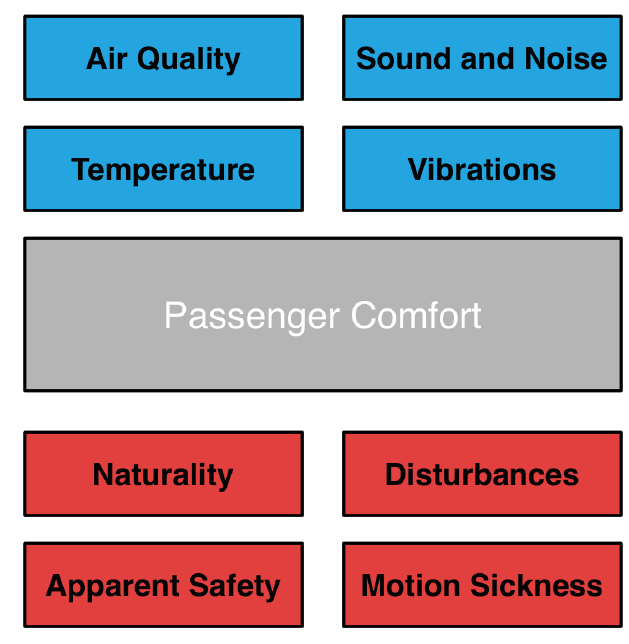
\includegraphics[width=0.48\textwidth]{comfort.PNG}
%	\end{center}
%	\caption{Overview of comfort parameters in autonomous vehicle with old parameters (blue) and new ones (red).(Source: \cite{Elbanhawi2015})}
%	\label{fig:Comfort}
%\end{wrapfigure}
In the paper 'Investigating ride comfort measures in autonomous cars' \cite{Elbanhawi2015}, it is explained that due to the introduction of autonomous vehicles there will be an other perception of comfort. Figure \ref{fig:Comfort} indicates in blue the claimed traditional comfort factors and in red the new ones that also have to be taken into account in when driving in autonomous vehicles. Concretely this can be translated into the preference of smooth trajectories and low lateral motions when the roads are assumed to be sufficiently smooth. A hypotheses is that motion sickness will be more prominent in autonomous driving due to the loss of control. Is is also argued that the amount of travel time and the distance to an obstacle are naturally parameters that contribute to a comfortable feeling. \\

In 'Analysis of Driving Style Preference in Automated Driving' \cite{Bellem} three studies are conducted in order to capture the definition of comfortable driving in autonomous vehicles.
In the first study drivers drove manually with their own driving styles and this data was used in order to look for relevant metrics that could be used in defining distinct driver styles. It was found that these metrics are varying across the maneuver. This is a logical result because not in all maneuvers are all the comfort matrices equally dominant.\\
The results of this research is that accelerations play a key role in comfort but are not the only factor. \cite{Bellem}\\

\begin{quote}
	The different comfort metrics found:
	\begin{itemize}
		\item lateral and longitudinal acceleration;
		\item lateral and longitudinal jerk;
		\item quickness of maneuver;
		\item headway distance;
	\end{itemize}
\end{quote}

Quickness of completing a lane change or an acceleration maneuver could respectively be modelled as: $q_L = \frac{\frac{\int velocity\cdot dt}{Time}}{\Delta distance}$ and $q_A = \frac{\frac{\int acceleration\cdot dt}{Time}}{\Delta velocity}$.\\

Comfortable driving as being assessed in \cite{Bellem} can be summarized as driving with small accelerations and jerk to obtain sufficient smooth trajectories and keeping sufficient headway distance in order to have a feeling of control and safety. These results suggest that when an algorithm to assess comfort is suggested for autonomous vehicles, a notion of the surrounding traffic should be inherently present. It was found that in order of the traffic density the driver is more tolerant towards less smooth driving behaviour e.g. to be able to insert in a busy lane. In this case higher comfort can be attained if the driver has a feeling of a fast responds of the vehicle translating in early peaks of acceleration. Vertical vibrations come not into scope when roads are assumed sufficiently smooth.\\

In a second study the main metrics that were found from study one are varied and combinations are rated by the use of a survey about the amount of comfort. "Out of this it followed that accelerations are playing a key factor." \cite{Bellem} For lane changes it could be concluded that the maneuvers with a small lateral acceleration and early perceivable onset were more comfortable. It is further also hypothesised that the location of the acceleration peaks and the amount of symmetry of the acceleration signal also plays a role when the amount of comfort is rated.\\

The relation between jerks and comfort is also confirmed by \cite{Gianna1996} where it is stated that: "Jerk has been shown to elicit a stronger influence on comfort than acceleration".


% In mijn maneuver wordt de kleine waardes van longitudinale snelheid en versnellingen gecompenseerd door de normalisatie waarden. Dus ookal zijn ze klein, krijgen toch een grote impact mee in het berekenen van een optimale oplossing. Daarin tegen kan er wel makkelijker voldaan worden aan het perfect voldoen van de longitudinale parameters in de lane change zonder het algemene resultaat veel te veranderen. De keuzen van de wegingsfactoren worden hierdoor minder significant en sensitiviteit wordt lager. --> als verschillende maneuvers worden gecombineerd zal dit de uniekheid van de gevonden wegingsfactoren opdrijven.


\subsection{Conclusion}
%Zie quotes van de slides!
In order to find parameters of driving comfort that will further on in the thesis will be used as comfort criteria, a literature study is conducted which is mainly questionnaire based. The results are that in order to be able to assess comfort higher order kinematic variables as accelerations and jerks should be taken into account. These are important variables in order to obtain a smooth vehicle path and to give a continuous and natural feeling when driving. Also should the quickness of the maneuver and the feeling of safety of the driver be taken into account. As quoted by \cite{Turner1999} states that low frequency lateral acceleration are the mean responsible for carsickness. In addition comfort assessment is influenced by the environment because in busier traffic there is a higher tolerance for less smooth trajectories. It was also found that the effect of a fast reaction of vehicle at the start of a maneuver is influencing the amount of comfort perceived in a positive way.


\section{Inverse reinforcement learning}
Because every human has its own driving style it is a cumbersome task to tune these parameters for each individual in order to model a personal perception of comfort. In \cite{Powers} it is showed that manual tuned parameters will lead besides also to sub-optimal solutions in comparison when the parameters are learned.  That is why it is chosen in this thesis to derive these parameters by demonstration of a human driver.\\

The goal of the learning algorithm explained in this thesis is to derive the parameters of different linearly combined comfort criteria combined in the costfuntion $J$ that when optimized as best as possible explain the observed data. As the match with the observed  data gets better, the model as suggested by equation \ref{eq:1} is getting closer to the inner comfort model of the individual driver. However it should be noted that the driver is taken unknowingly a lot of comfort criteria into account and they are not always linearly relating. Therefore the suggested comfort cost function consisting of a linear combination of comfort criteria will always be an approximation of the reality. Yet as discussed in \cite{Kuderer2015a} the results suggest that the magnitudes of the quantities that contribute to the comfort of the user are obtained.\\

\begin{equation}\label{eq:1}
	J = \sum_{j=1}^{N}\theta_j\cdot f_j	
\end{equation}

%"Inverse optimal control, also known as inverse reinforcement learning, is the problem of recovering an unknown reward function in a Markov decision process from expert demonstrations of the optimal policy." \cite{Levine2012} In contrary what this classic definition, the approach followed by \cite{Kuderer2015a} is not modelling teh


In order to create a generative model that create vehicle paths $r_i$ with equivalent kinematic characteristics as the path that was observed $\tilde{r_i}$, a feature-based inverse reinforcement learning is applied. \cite{Kuderer2015a,Abbeel2004} With $i \in [1 ... m]$ and $m$ the amount of observed trajectories. A feature is encoding relevant kinematic properties and the difference between the demonstrated and calculated features says something about the similarity of the kinematic vehicle signals. \\

\subsection{Background on learning algorithm}
A feature values maps a trajectory onto a scalar and the higher the scalar value the more discomfort is experienced. An example of a that measures the amount of accelerations in a maneuver is given by equation \ref{eq:3}.

\begin{equation}\label{eq:3}
f:\bm{r}\xrightarrow{}f(\bm{r})=\int_{0}^{T}\ddot{x}(t)^{2}+\ddot{y}(t)^{2} dt
\end{equation}

The path that that the centre of gravity of the vehicle is following can be represented by: \ref{eq:4}.
\begin{equation}\label{eq:4}
\bm{r}:t \xrightarrow{}\bm{r}(t) =  \bigl( \begin{smallmatrix} x(t)\\ y(t) \end{smallmatrix}\bigr)
\end{equation}

The driver is not a deterministic agent and is modelled by a stochastic distribution: $p(\bm{r}|\bm{\theta})$ For certain weights $\bm{\theta} \in \mathbb{R}^N$ a path $\bm{r}$ is produced as being a sample of a stochastic distribution. The distribution that is chosen for this is the distribution of maximum entropy (equation: \ref{eq:entropy}). \cite{Ziebart2008, Kretzschmar2014}. This describes the data best because it is the distribution that is least biased. \cite{Kuderer2015a} 
The distribution with the highest entropy represents the given information best since it does not favour any particular outcome besides the observed constraints. \cite{Abbeel2004}
	
	
\begin{equation}\label{eq:entropy}
	p(\bm{r}|\bm{\theta}) = exp(-\bm{\theta}^T\cdot \bm{F}(\bm{r}))
\end{equation}
Equation \ref{eq:entropy} can be interpreted as a linear costfunction $\bm{\theta}^T\bm{F}(\bm{r})$ where agents are exponentially more likely to select trajectories with lower cost. \cite{Kuderer2015a}
The observed feature vector $\tilde{\bm{F}} \in \mathbb{R}^N$ has on its entries the different feature values $\tilde{f_i}$ with $i \in [1...m]$. The averaged observed feature vector is $\tilde{\bm{F}}_{av} = \frac{1}{m}\sum_{j=1}^{m}\tilde{\bm{F}_j}$.\\

In order to be able to explain the averaged observed feature vector, the weights $\bm{\theta}$ need to be found that match the expected features vector obtained from the distribution $\bm{F}(r_{expected})$ with the averaged observed features vector $\bm{F}_{obs}$. $\bm{r}_{expected}$ defined as $ E(p(\bm{r}|\bm{\theta}))$. To make the expected features vector match the averaged observed features vector, gradient descent method can be used with as gradient $\bm{F}_{obs} - \bm{F}(r_{expected})$. Equation \ref{eq:5} summarizes the gradient descent method with $\alpha$ the step size taken in the direction of descent.
\begin{equation}\label{eq:5}
	\bm{\theta}^{k+1} = \bm{\theta}^{k} - \alpha \pdv{\bm{F}}{\bm{\theta}}^k 
\end{equation}

When $\bm{\theta}_{optimal}$ is found the gradient is minimized and the features vectors will match as closely as possible. "When the feature expectations match, guaranteeing that the learner performs equivalently to the agent's demonstrated behaviour regardless of the actual reward weights the
agent is attempting to optimize" \cite{Abbeel2004}\\

In order to calculate $\bm{F}(\bm{r}_{expected})$ a Hamiltonian Markov chain
Monte Carlo stochastic distribution sampling approached is used in \cite{Kretzschmar2014}. In \cite{Kuderer2015a} a simplified method and less calculation demanding approach is proposed where it is assumed that the expected path is the one that is been assessed as the most comfortable by the driver and is thus the path that is minimizing \ref{eq:1} for certain weights. In order to be able to match with the observed data it is hereby assumed that the demonstrations not only are samples of a stochastic distribution but are also generated by optimizing an inner cost function which is similar to \ref{eq:1}. Equation \ref{eq:6} summarizes the approximation proposed by \cite{Kuderer2015a}.
\newcommand{\argmax}{argmax}
\newcommand{\argmin}{argmin}

\begin{equation}\label{eq:6}
	\bm{r}_{expected} = \underset{\bm{r}}{\argmax} \hspace{1mm} p(\bm{r}|\bm{\theta}) = \underset{\bm{r}}{\argmin} \hspace{1mm}  \bm{\theta}^T\cdot \bm{F}(\bm{r})
\end{equation}
\begin{equation}\label{eq:new}
	\pdv{\bm{F}}{\bm{\theta}} = \bm{F}_{obs} - \bm{F}(\bm{r}_{expected})
\end{equation}


%\DeclareMathOperator*{\argmin}{argmin}
It is checked in chapter \ref{cha:Learning_algorithm} if this approach that is assuming that demonstrations are generated by minimizing a cost function also gives acceptable results when the assumption is violated.

\subsection{RPROP algorithm}\label{s:RPROP}
From \cite{Panos_opti} it is known that not every step size in the opposite direction of the gradient is leading to the convergence towards a minimum. When the step size is too small it will take a long time to convergence. However when it is chosen too big, cycling behaviour between limit points can occur. In order to avoid this kind of unwanted behaviour a line-search method is needed in order to change the step size taken during the course of the algorithm. For this the Resilient backpropagation algorithm (\textbf{RPROP}) \cite{RPROP} is used as it was first proposed by Martin Riedmiller and Heinrich Braun in 1993.\\

The main advantage when using RPROP is that the size of the gradient is not blurring the update value of the weights for the start of the next iteration in the gradient descent optimization method. The update value $\Delta u$ is solely dependent of the sign of the current gradient and the sign of the gradient in the previous iteration. The main equations of the algorithm are given for each by: 

\begin{equation}\label{eq:7}
	\Delta u^t_i =
	\begin{Bmatrix}
		 \eta^+ \cdot \Delta u^{t-1}_i, & if \hspace{1 mm} \pdv{f_i}{\theta_i}^t \cdot \pdv{f_i}{\theta_i}^{t-1} > 0 \\
		 \eta^- \cdot \Delta u^{t-1}_i, & if \hspace{1 mm} \pdv{f_i}{\theta_i}^t \cdot \pdv{f_i}{\theta_i}^{t-1} < 0 \\
		  \Delta u^{t-1}_i, & if \hspace{1 mm} \pdv{f_i}{\theta_i}^t \cdot \pdv{f_i}{\theta_i}^{t-1} = 0 \\
	\end{Bmatrix}
\end{equation}

When the update value of the weight is determined it is applied in the direction of steepest descent which equals the opposite direction of the current gradient. 

\begin{equation}\label{eq:8}
\Delta \theta^t_i =
\begin{Bmatrix}
	-\Delta u^t_i, & if \hspace{1 mm} \pdv{f_i}{\theta_i}^t > 0 \\
	+ \Delta u^t_i, & if \hspace{1 mm} \pdv{f_i}{\theta_i}^t < 0 \\
	0, & else 
\end{Bmatrix}
\end{equation}
Exception on \ref{eq:8}:

\begin{equation}\label{eq:10}
	\Delta \theta^t_i = -\Delta \theta^{t-1}_i, \hspace{1mm} if \hspace{1mm} \pdv{f_i}{\theta_i}^t \cdot \pdv{f_i}{\theta_i}^{t-1} < 0
\end{equation}

\begin{equation}\label{eq:9}
	0 <\eta^-<1<\eta^+
\end{equation}

and with $\theta_i^{t+1} = \theta_i^{t} + \Delta \theta^t_i$, $i \in \mathbb{N}_{[1\cdots N]}$ and $t \in \mathbb{N}_[1 \cdots \mathbb{\tau}]$ the amount of iterations. Every time the partial derivative $\pdv{f_i}{\theta_i}^t$ of the corresponding weight $\theta_i^t$ changes its sign, it is assumed that the last update was too big and the local minimum was passed. In \ref{eq:7} the step size is reduced and in order to go back the previous situation the update of the weight is done as \ref{eq:10}. In order to not again decrease the update value when going back to the previous situation, in the next iteration $\pdv{f_i}{\theta_i}^{t-1}$ is set equal to zero.\\
If the derivative retains its sign, the update-value is slightly increased in order to accelerate convergence in shallow regions." \cite{RPROP} Parameters chosen bij the user are $\Delta_0, \eta^+$ and $\eta^-$. In this thesis following values were chosen: $\Delta_0 = 0.1$, $\eta^+ = 1.2$ and $\eta^- = 0.5$.

\subsection{Optimization principles}
The optimization tool used is the CasADi software. This section discusses the main optimization principles used under the hood and discusses the IPOPT solver and SQP method. (See Handbook opti and slides CasADi 3 lecture vooral)


%--> in main paper they make the assumption of calculating most likely path --> features expected = f(r_exp) instead of sampling as is done in this paper.
%(Hamiltonian Markov chain Monte Carlo methods = very computation expensive)
%



%When the averaged observed feature vector $F$
%
%In order to be able to explain the observed trajectory
%
% Firstly he is generating observed paths that are a sample of a distribution and secondly he is minimizing its own comfort cost function.
%
% 
%The exponential distribution is giving a higher chance to produce paths that have a low feature value associated  with a high weight factor. This means that the more influence a feature value has on the total amount of comfort (higher weight), how less likely it becomes that the driver will produce a certain path that will trigger a high value of the concerned feature value. 
%
%If you maximize the probability you get the most likely expected path for the chosen weights.  This can be translated in the assumption that the driver is most likely to produce a path that will be experienced as comfortable as possible by himself. The assumption that the driver is optimizing its own comfort cost function is an assumption on top of assuming that the observed path is a sample of an exponential distribution with certain weight factors. 
%
%The goal of the learning process is to learn the model parameters (weight factors) of the driver from their observed driving style. It is assumed that the driver can be explained by a probability distribution and that it produces paths that minimize a comfort cost function. When the comfort model of the driver is learned, it can be further used in general situations. This is done by implementing the user specific notion of comfort in the motion planning algorithm of a model predictive control planning application.
%
%The learned model should produce trajectories that are similar in order of comfort as experienced by the driver. This is a logical consequence because the model is derived from the observed data. The difference between the features of the observed and generated paths quantify the similarity and at convergence of the learning algorithm, the feature values are as close as possible. As close as possible should be taken with a grain of salt though. This can be explained by making a comparison between the curvature and the jerk where curvature is in order of 10^-5 and jerk is in order of 10^2. This means that a difference of 1 has a far more bigger impact on curvature than on jerk and normalization is necessary. Normalization is done by dividing the calculated features by their corresponding observed feature value in order to make it dimensionless.  This means that the optimization should be done without fixing time! The difference in feature values is the driving factor and this will indirect specify also the time of the lane change.
%
%Learning a model implies finding the best suitable values of the tunable parameters which are in this case the weight factors. To summarize, the goal of the learning algorithm is to find the weight factors which give the smallest difference between the feature values of the observed path and the feature values of the calculated path, which is the path that minimizes the linear comfort cost function. The calculated path is generated by the minimization of the comfort cost because minimizing the comfort cost function is equal to maximizing the exponential distribution and the resulting path is equal to the most likely generated path for certain weight factors. The most likely generated path is compared with the observed one. With this it is indirectly assumed that the observed paths are generated by a human driver that is minimizing its own unknow comfort cost function. It will be clear from the validation in chapter \ref{} if this assumption holds. From [hoofdrapport] it is assumed that this approximation is suitable in the context of learning individual driving styles on highways.  Two assumptions apply on the human driver. Firstly he is generating observed paths that are a sample of a distribution and secondly he is minimizing its own comfort cost function. It should be noted that in practice instead of using personal data also data form an expert driver can be made available to the user. This to avoid bad autonomous behavior as a result of an inexperienced human driver.
%
%
%Note that the features of the path that are obtained by minimizing the comfort cost function should be possible to converge to the features of the observed path. The driver that is producing the observed path is assumed to maximize its personal comfort when generating the observation data which means that the most personal comfort is attained when the difference between the feature values of the observed and calculated paths are small. (this should be normalized) 
%


\subsubsection{Conclusion}
A background from literature on the inverse reinforcement learning algorithm used in this thesis was given. First inverse reinforcement learning was explained and how it could help to solve the research question how to learn comfort from observations. Afterwards a more detailed background on the formulation of the specific learning algorithm was given, which was complemented with a discussion on the algorithm used to update the weights being part of the gradient descent method to match expected feature values with observed ones.
\newpage


%\section{bekijk hiervoor de andere approaches - to be read further}
%
%\subsection{Machine learning approach}
%\subsection{paper brecht approach}

%Dan komt de vraag wat is comfort precies? Literatuur studie...
%Waarnaar kan men kijken als men het over comfort heeft. 
%Lane change bekeken om comfort te valideren --> zeg dat er geen iso standaarden aanwezig zijn.
%Hoe wordt een bestuurder gemoddelleerd --> dit wordt gedaan door een kansverdeling.
%Waarom is entropie nuttig om deze bestuurder te kunnen bekijken? Doe hier meer ondezoek over en verantwoord het gebruik hiervan. Conclusie komt af met comfort parameters die verder worden gebruikt als features.
%Bij de uitleg van de features en waarom er versnelling en acceleratie wordt gebruikt, basseer ook op paper 7 van hoofdpaper--> geen acces
%
%Wat wordt er in de literatuur al gebruikt om comfort te modelleren en geef een overzicht.
%
%Leg uit hoe komt aan entropy distribution komt --> kan beroep doen op ref 2 en 20 van het hoofdrapport (both are assuming an exponential distribution) (IMPORTANT) --> literatuur study niet te uitgebreid maken...
%
%Check uitgebreide samenvatting van hoofdpaper op oneNote.
%
%Dit is de reden voor het gebruik van de maximum entropie distributie: 
%	To learn observed behavior, we aim to model the distribution
%	that underlies the empirical sample trajectories.
%	Following Abbeel and Ng [1], we aim to find a model that
%	induces distributions that match, in expectation, the feature
%	values fD of the empirical trajectories D, yielding
%	Ep(x)[f (x)] = fD =
%	1
%	jDj
%	X
%	xk2D
%	f (xk): (1)
%	In general, however, there is not a unique distribution that
%	matches the features. Ziebart et al. [24] resolve this ambiguity
%	by applying the principle of maximum entropy [10], which
%	states that the distribution with the highest entropy represents
%	the given information best since it does not favor any
%	particular outcome besides the observed constraints. (this is the least baised distribution)
%	Modelling expected featueres by hybrid monte carlo method: https://reader.elsevier.com/reader/sd/pii/037026938791197X?token=71567B7640C402F2FF578E34E3BB7914CA14E4A1A29DE88D9534D96C9305E13DA52D0424FF1475A822FCE784725196D3
%%	ref: C:\Users\t2vosx\OneDrive\Documenten\Leuven\Thesis\References2\Citations on main %paper\Learning to Predict Trajectories of Cooperatively Navigating Agents.pdf>
%
% 	paper: Feature-based prediction of trajectories for socially compliant navigation
%	which
%	states that the distribution with the highest entropy represents
%	the given information best since it does not favor any
%	particular outcome besides the observed constraints.
	
%	• Weet dat exponentiële vorm oplossing is van boven staand optimizatie probleem. zie foto
%	--> volgt uit FONC --> oplossing moet (non convex) voldoen aan KKT conditions. Er zijn enkel maar equality constraints aanwezig --> primal feasibility en lagrange stationarity moeten voldaan worden --> LS wordt gecontroleerd drm van de Euler - lagrange vergelijking te gebruiken. 


%%% Local Variables: 
%%% mode: latex
%%% TeX-master: "thesis"
%%% End: 
